\documentclass[12pt,a4paper]{report}

% -------------------- Packages --------------------
\usepackage[utf8]{inputenc}
\usepackage[T1]{fontenc}
\usepackage{newtxtext,newtxmath}
\usepackage[a4paper,margin=1in]{geometry}
\usepackage{setspace}
\usepackage{graphicx}
\usepackage{float}
\usepackage{booktabs}
\usepackage{array}
\usepackage{amsmath,amssymb}
\usepackage{enumitem}
\usepackage{hyperref}
\usepackage{xcolor}
\usepackage{tikz}
\usepackage{caption}
\usepackage{longtable}
\usepackage{listings}
\usetikzlibrary{arrows.meta,positioning,shapes.geometric,fit}

\onehalfspacing
\setlength{\parindent}{1.25cm}
\setlength{\parskip}{3pt}
\setlist[itemize]{leftmargin=1.5em,itemsep=2pt,topsep=3pt}
\setlist[enumerate]{leftmargin=1.7em,itemsep=2pt,topsep=3pt}
\hypersetup{
    colorlinks=true,
    linkcolor=black,
    citecolor=black,
    urlcolor=blue,
    pdftitle={Dynamic Layer Adaptation and Guided Weight Adaptation},
    pdfauthor={RGUKT Nuzvid CSE Project Team}
}

% -------------------- Editable project details --------------------
\newcommand{\ProjectTitle}{DYNAMIC LAYER ADAPTATION (DLA) AND GUIDED WEIGHT ADAPTATION (GWA)}
\newcommand{\ProjectSubtitle}{Avoiding Catastrophic Forgetting while Adapting to New Domains}
\newcommand{\University}{Rajiv Gandhi University of Knowledge Technologies -- Nuzvid}
\newcommand{\Department}{Department of Computer Science and Engineering}
\newcommand{\GuideName}{K.K. Sing}
\newcommand{\PanelName}{Maha Lakshmi Rao}

% -------------------- Document --------------------
\begin{document}

% =========================================================
% TITLE PAGE
% =========================================================
\begin{titlepage}
\thispagestyle{empty}
\begin{center}
\vspace*{0.35cm}
{\Large\bfseries \ProjectTitle}\\[0.35cm]
{\large\bfseries \ProjectSubtitle}\\[1.0cm]

{\large A Project Report}\\[0.35cm]
Submitted in partial fulfillment of the requirements for the award of the degree of\\[0.35cm]
{\Large\bfseries BACHELOR OF TECHNOLOGY}\\[0.25cm]
in\\[0.25cm]
{\Large\bfseries COMPUTER SCIENCE AND ENGINEERING}\\[0.9cm]

Submitted by\\[0.35cm]
\begin{tabular}{ll}
\textbf{K. Vishal Kathik} & \textbf{N210037}\\
\textbf{R. Praneetha} & \textbf{N210477}\\
\textbf{K. Ramya} & \textbf{N210627}\\
\textbf{Santhosh} & \textbf{N21000}\\
\end{tabular}

\vspace{0.8cm}
Under the esteemed guidance of\\[0.2cm]
{\large\bfseries \GuideName}\\[0.65cm]

\IfFileExists{rguktn.png}{
    \includegraphics[width=0.19\textwidth]{rguktn.png}
}{
    \fbox{\parbox[c][2.1cm][c]{3.2cm}{\centering Insert\\RGUKT logo}}
}\\[0.55cm]

{\large\bfseries \Department}\\[0.2cm]
{\large \University}\\
Nuzvid, Andhra Pradesh -- 521202\\[0.25cm]
{\large Academic Year 2026--2027}
\end{center}
\end{titlepage}

% =========================================================
% CERTIFICATE OF COMPLETION
% =========================================================
\pagenumbering{roman}
\chapter*{CERTIFICATE OF COMPLETION}
\addcontentsline{toc}{chapter}{Certificate of Completion}

\begin{center}
\IfFileExists{rguktn.png}{\includegraphics[width=0.16\textwidth]{rguktn.png}\\[0.3cm]}{}
{\bfseries \Department}\\
\University\\
Nuzvid, Andhra Pradesh -- 521202\\[0.7cm]
{\Large\bfseries CERTIFICATE OF COMPLETION}
\end{center}

This is to certify that the project report entitled
\textbf{``\ProjectTitle: \ProjectSubtitle''} is the bonafide work of
\textbf{K. Vishal Kathik (N210037), R. Praneetha (N210477),
K. Ramya (N210627), and Santhosh (N21000)}, carried out under the
guidance and supervision of \textbf{\GuideName} in partial fulfillment
of the requirements for the award of the degree of Bachelor of Technology
in Computer Science and Engineering at RGUKT Nuzvid during the academic
year 2026--2027.

\vspace{1.6cm}
\noindent
\begin{minipage}{0.47\textwidth}
\centering
\rule{6cm}{0.4pt}\\
\textbf{\GuideName}\\
Project Guide
\end{minipage}
\hfill
\begin{minipage}{0.47\textwidth}
\centering
\rule{6cm}{0.4pt}\\
\textbf{Head of the Department}\\
Department of CSE
\end{minipage}

\vspace{1.2cm}
\noindent Place: Nuzvid \hfill Date: \rule{3cm}{0.4pt}

% =========================================================
% CERTIFICATE OF EXAMINATION
% =========================================================
\clearpage
\chapter*{CERTIFICATE OF EXAMINATION}
\addcontentsline{toc}{chapter}{Certificate of Examination}

\begin{center}
\IfFileExists{rguktn.png}{\includegraphics[width=0.16\textwidth]{rguktn.png}\\[0.3cm]}{}
{\bfseries \Department}\\
\University\\
Nuzvid, Andhra Pradesh -- 521202\\[0.7cm]
{\Large\bfseries CERTIFICATE OF EXAMINATION}
\end{center}

This is to certify that the project report entitled
\textbf{``\ProjectTitle: \ProjectSubtitle''}, submitted by
\textbf{K. Vishal Kathik (N210037), R. Praneetha (N210477),
K. Ramya (N210627), and Santhosh (N21000)}, has been examined and is
approved as a project work presented in partial fulfillment of the
requirements for the award of the degree of Bachelor of Technology in
Computer Science and Engineering.

The approval of this report does not necessarily imply acceptance of
every statement, opinion, or conclusion expressed in it. It signifies
acceptance of the work for the purpose for which it has been submitted.

\vspace{1.5cm}
\noindent
\begin{minipage}{0.47\textwidth}
\centering
\rule{6cm}{0.4pt}\\
\textbf{\GuideName}\\
Project Guide
\end{minipage}
\hfill
\begin{minipage}{0.47\textwidth}
\centering
\rule{6cm}{0.4pt}\\
\textbf{\PanelName}\\
Panel Examiner
\end{minipage}

\vspace{1.1cm}
\noindent Place: Nuzvid \hfill Date: \rule{3cm}{0.4pt}

% =========================================================
% DECLARATION
% =========================================================
\clearpage
\chapter*{DECLARATION}
\addcontentsline{toc}{chapter}{Declaration}

We hereby declare that the project report entitled
\textbf{``\ProjectTitle: \ProjectSubtitle''} is the result of the work
carried out by us under the guidance of \textbf{\GuideName},
\Department, RGUKT Nuzvid. This report is submitted in partial fulfillment
of the requirements for the award of the degree of Bachelor of Technology
in Computer Science and Engineering.

We further declare that this work is our own and that all material
obtained from other sources has been appropriately acknowledged and cited.
To the best of our knowledge, this report has not been submitted, either
in full or in part, to any other institution for the award of a degree
or diploma.

\vspace{1cm}
\noindent Place: Nuzvid\\
Date: \rule{3cm}{0.4pt}

\vspace{1cm}
\begin{flushright}
\begin{tabular}{ll}
\textbf{K. Vishal Kathik} & (N210037)\\[0.2cm]
\textbf{R. Praneetha} & (N210477)\\[0.2cm]
\textbf{K. Ramya} & (N210627)\\[0.2cm]
\textbf{Santhosh} & (N21000)
\end{tabular}
\end{flushright}

% =========================================================
% ACKNOWLEDGEMENT
% =========================================================
\clearpage
\chapter*{ACKNOWLEDGEMENT}
\addcontentsline{toc}{chapter}{Acknowledgement}

We express our sincere gratitude to our project guide,
\textbf{\GuideName}, for the guidance, valuable suggestions, and
encouragement provided throughout this project. The discussions and
feedback helped us develop and evaluate the proposed approaches.

We also thank \textbf{\PanelName} for the valuable observations and
suggestions during the project review. We are grateful to the faculty
members of the \Department, RGUKT Nuzvid, for their support and for
providing the academic environment and resources required to carry out
this work.

Finally, we thank our families and friends for their encouragement and
support throughout the completion of this project.

% =========================================================
% ABSTRACT
% =========================================================
\clearpage
\chapter*{ABSTRACT}
\addcontentsline{toc}{chapter}{Abstract}

Deep learning models are often adapted to a new task by fine-tuning their
parameters on a new dataset. However, updating a large portion of a
pretrained network can alter previously learned representations and may
lead to \emph{catastrophic forgetting}, in which performance on the
original domain degrades after learning the new domain. This project
studies two parameter-selection strategies intended to restrict the
updates made during adaptation: \textbf{Dynamic Layer Adaptation (DLA)}
and \textbf{Guided Weight Adaptation (GWA)}.

DLA selects either one or two complete layers of a four-layer
convolutional neural network at each iteration. The selected layers are
trainable while the remaining feature-extraction layers are frozen.
GWA selects approximately ten percent of the parameters independently
within each of the four stages of a pretrained ResNet-18. Gradient masks
are used so that only the selected parameter elements receive updates.
For both supplied implementations, CIFAR-100 is used as the training
dataset and MiniImageNet is used for evaluation. The training procedure
runs for five epochs per iteration, with a maximum of forty iterations
and early stopping based on the CIFAR-100 validation accuracy.

The evaluation considers CIFAR-100 classification accuracy and
MiniImageNet accuracy, together with KL divergence and prediction
agreement relative to the corresponding initial reference model.
The comparative values recorded in the project presentation report
CIFAR-100 accuracies of 76.37\% for DLA and 75.96\% for GWA, with
prediction-agreement values of approximately 79\% for both methods.
These values are reported presentation results and should be associated
with the exact experiment configuration that produced them.

The project explores whether changing the trainable subset over
successive iterations can provide a practical way to control parameter
updates during domain adaptation. It also highlights the importance of
using consistent model initialization and evaluation heads when making
a scientifically valid comparison of forgetting across methods.

% =========================================================
% TABLE OF CONTENTS
% =========================================================
\clearpage
\tableofcontents
\clearpage
\listoffigures
\listoftables

% =========================================================
% MAIN MATTER
% =========================================================
\clearpage
\pagenumbering{arabic}

\chapter{Introduction}

\section{Overview}
Deep neural networks learn useful feature representations from large
datasets. A model trained on one domain can often be adapted to another
domain through fine-tuning. Although this can improve performance on the
new task, unrestricted updates may modify parameters that are important
for the original task. This degradation of previously acquired
capabilities is commonly known as catastrophic forgetting.

This project investigates two ways of restricting the trainable
parameters during adaptation. DLA changes the set of trainable layers
between iterations, whereas GWA changes the selected parameter elements
within each network stage. The experiments use CIFAR-100 as the target
training dataset and MiniImageNet as the evaluation dataset for
monitoring the behaviour of the model on the other domain.

\section{Motivation}
The main motivation is to investigate whether limiting the parameters
updated during fine-tuning can reduce unnecessary changes to previously
learned representations. Conventional full fine-tuning updates all
trainable backbone parameters. This gives the model considerable
flexibility, but it can also cause substantial parameter drift.

Parameter-efficient approaches such as adapters and low-rank updates
restrict the trainable capacity, but generally use a predefined
parameterization. The approaches studied in this project instead
investigate dynamically changing the trainable subset:
\begin{itemize}
    \item \textbf{DLA:} selects one or two complete feature-extraction
    layers at each iteration.
    \item \textbf{GWA:} selects approximately ten percent of the
    parameters independently in each stage and applies gradient masks.
\end{itemize}

The motivation is to compare coarse-grained layer selection with
fine-grained parameter selection under an iterative training procedure.

\section{Problem Statement}
Given a model with parameters $\theta$ initially associated with a
reference domain, the objective is to adapt the model to a target dataset
while monitoring changes in its behaviour on the reference evaluation
domain. Instead of updating every backbone parameter at every iteration,
the methods construct a trainable subset $S_t$ at iteration $t$.

The optimization can be expressed as
\[
\theta_{t+1} =
\theta_t - \eta\, M_t \odot \nabla_{\theta}\mathcal{L}_{\mathrm{target}},
\]
where $M_t$ is a binary update mask, $\eta$ is the learning rate,
$\odot$ denotes element-wise multiplication, and
$\mathcal{L}_{\mathrm{target}}$ is the target-task loss. For DLA,
$M_t$ is defined by the selected complete layers. For GWA, it is
defined by the selected parameter elements within each stage.

\section{Objectives}
The objectives of this project are:
\begin{enumerate}
    \item To study catastrophic forgetting during adaptation from an
    original domain to a new domain.
    \item To implement DLA using dynamic selection of one or two
    complete CNN layers per iteration.
    \item To implement GWA using random selection of approximately
    ten percent of the parameters in each ResNet-18 stage.
    \item To train the models on CIFAR-100 and evaluate their behaviour
    on MiniImageNet.
    \item To measure target-task accuracy, reference-domain accuracy,
    KL divergence, and prediction agreement.
    \item To compare the two parameter-selection strategies and identify
    limitations that should be addressed in future experiments.
\end{enumerate}

\section{Contributions}
The work makes the following contributions:
\begin{itemize}
    \item A dynamic layer-selection training procedure that resamples
    the selected CNN layers at each iteration.
    \item A guided weight-selection procedure that creates per-stage
    binary masks and uses gradient hooks to restrict parameter updates.
    \item A common evaluation design based on target accuracy and
    reference-model behaviour.
    \item An experimental comparison of coarse-grained and
    fine-grained parameter selection, together with an examination of
    implementation constraints.
\end{itemize}

\chapter{Related Works}

\section{Elastic Weight Consolidation}
Kirkpatrick et al. introduced Elastic Weight Consolidation (EWC), which
uses an estimate of parameter importance based on the Fisher
information matrix to penalize changes to parameters that are important
for previously learned tasks \cite{ewc}. EWC is related to this project
because both approaches aim to reduce destructive parameter changes.
Unlike EWC, DLA and GWA restrict which parameters are updated at a
particular iteration rather than adding an importance-weighted
regularization penalty.

\section{PackNet}
PackNet uses iterative pruning and parameter freezing to make room for
new tasks while preserving parameters assigned to earlier tasks
\cite{packnet}. The idea of controlling which weights remain trainable
is related to the parameter-selection mechanism used in GWA.

\section{Progressive Neural Networks}
Progressive Neural Networks preserve previously learned network columns
and add new capacity for new tasks \cite{progressive}. This provides
another strategy for reducing interference between tasks. The methods
in this project do not add new network columns; they reuse the existing
network and dynamically select its trainable components.

\section{Low-Rank Adaptation}
LoRA adapts pretrained models by learning low-rank update matrices
while keeping the original weights fixed \cite{lora}. It is a
parameter-efficient fine-tuning method. GWA also limits the number of
updated parameters, but does so by selecting parameter elements from
existing network stages.

\section{Adapters}
Adapters introduce small trainable modules into a mostly frozen
pretrained network \cite{adapters}. They provide a fixed structural
mechanism for parameter-efficient adaptation. DLA and GWA instead
change the selected trainable components during the iterative process.

\section{Lottery Ticket Hypothesis}
The Lottery Ticket Hypothesis investigates whether sparse subnetworks
within a larger neural network can be trained effectively
\cite{lottery}. It motivates the study of sparse parameter subsets.
GWA uses a changing random subset rather than identifying one
fixed winning subnetwork.

\section{Research Gap}
The reviewed methods demonstrate several ways to reduce interference
between tasks, including regularization, pruning, architectural
expansion, and parameter-efficient modules. This project investigates
a complementary strategy: dynamically resampling the trainable subset
during adaptation. DLA performs this selection at the layer level,
whereas GWA performs it at the parameter-element level.

\chapter{Methodology}

\section{Experimental Setup}
The supplied implementations use the following principal settings.
Values are taken from the provided code files.

\begin{table}[H]
\centering
\caption{Main experimental configuration}
\begin{tabular}{p{0.42\textwidth}p{0.48\textwidth}}
\toprule
\textbf{Setting} & \textbf{Value}\\
\midrule
Target training dataset & CIFAR-100\\
Reference evaluation dataset & MiniImageNet\\
Input image size & $224\times224$\\
Batch size & 64\\
Epochs per iteration & 5\\
Maximum iterations & 40\\
Early-stopping patience & 3 iterations\\
Backbone learning rate & 0.0001\\
CIFAR classifier learning rate & 0.01\\
Optimizer & SGD, momentum 0\\
Weight decay & 0\\
Random seed & 42\\
\bottomrule
\end{tabular}
\end{table}

The training transforms resize images to $224\times224$, apply random
horizontal flipping during training, convert images to tensors, and
normalize them using the ImageNet channel mean and standard deviation.
The evaluation transforms use resizing, tensor conversion, and the
same normalization without random flipping.

\section{Dataset Description}
\subsection{CIFAR-100}
CIFAR-100 is used as the target dataset for training. It contains
100 object categories. The supplied code loads the training and test
folders using an image-folder dataset interface and checks that the
class mappings are consistent.

\subsection{MiniImageNet}
MiniImageNet is used by the supplied scripts for evaluation of the
reference-domain behaviour. The code maps folder class identifiers to
ImageNet class indices using the provided ImageNet class-index JSON
file. The evaluation script computes classification accuracy and
compares the updated model's predictions with predictions obtained
from the initial reference model.

\section{Model Architecture}

\subsection{DLA: Custom Four-Layer CNN}
The supplied DLA implementation uses a custom CNN consisting of four
convolutional blocks. Each block contains a convolution, batch
normalization, ReLU activation, and max-pooling operation.

\begin{table}[H]
\centering
\caption{Custom CNN feature extractor used in the DLA code}
\begin{tabular}{cccc}
\toprule
\textbf{Layer} & \textbf{Input channels} & \textbf{Output channels} & \textbf{Operations}\\
\midrule
Layer 1 & 3 & 32 & Conv, BN, ReLU, MaxPool\\
Layer 2 & 32 & 64 & Conv, BN, ReLU, MaxPool\\
Layer 3 & 64 & 128 & Conv, BN, ReLU, MaxPool\\
Layer 4 & 128 & 256 & Conv, BN, ReLU, MaxPool\\
\bottomrule
\end{tabular}
\end{table}

An adaptive average-pooling layer converts the final feature map into a
256-dimensional feature vector. A fully connected classifier maps this
vector to 100 CIFAR-100 classes. The code also defines a 1000-class
ImageNet evaluation probe.

\textbf{Implementation note:} In the supplied DLA code, the reference
CNN is randomly initialized, and the ImageNet probe is also randomly
initialized and frozen. The student model is copied from this same
initialization. Therefore, this particular implementation is not a
pretrained ImageNet model, and its MiniImageNet accuracy should not be
interpreted as retained pretrained ImageNet knowledge. This distinction
must be considered when interpreting or comparing DLA results.

\subsection{GWA: Pretrained ResNet-18}
The supplied GWA implementation loads ResNet-18 with pretrained
ImageNet weights. A copy of the pretrained network is used as the
student backbone. The original ImageNet fully connected classifier is
preserved as a frozen evaluation probe, while the backbone's original
classifier is replaced by a new 100-class CIFAR-100 classifier.

The four residual stages, \texttt{layer1}, \texttt{layer2},
\texttt{layer3}, and \texttt{layer4}, form the parameter groups from
which GWA selects trainable parameter elements. The ImageNet probe
remains frozen during CIFAR-100 training.

\subsection{Data Flow}
The overall data flow is summarized in Figure~\ref{fig:dataflow}.

\begin{figure}[H]
\centering
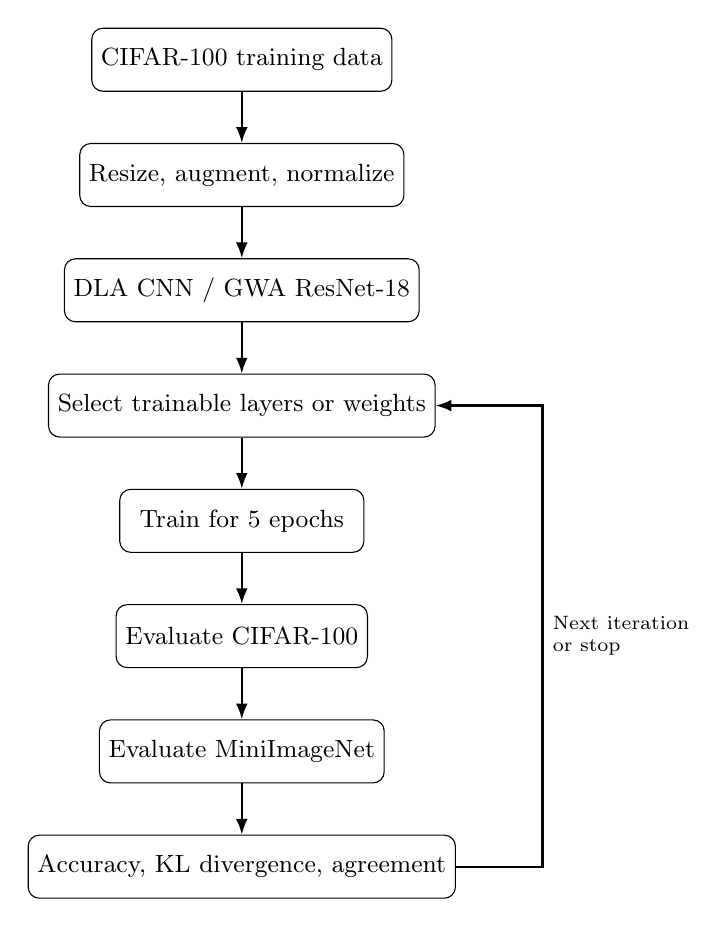
\begin{tikzpicture}[
    node distance=0.65cm and 0.9cm,
    box/.style={draw,rounded corners,align=center,minimum width=3.1cm,
                minimum height=0.8cm,font=\small},
    arrow/.style={-{Latex[length=2mm]},thick}
]
\node[box] (data) {CIFAR-100 training data};
\node[box,below=of data] (prep) {Resize, augment, normalize};
\node[box,below=of prep] (model) {DLA CNN / GWA ResNet-18};
\node[box,below=of model] (select) {Select trainable layers or weights};
\node[box,below=of select] (train) {Train for 5 epochs};
\node[box,below=of train] (eval) {Evaluate CIFAR-100};
\node[box,below=of eval] (mini) {Evaluate MiniImageNet};
\node[box,below=of mini] (metrics) {Accuracy, KL divergence, agreement};
\draw[arrow] (data)--(prep);
\draw[arrow] (prep)--(model);
\draw[arrow] (model)--(select);
\draw[arrow] (select)--(train);
\draw[arrow] (train)--(eval);
\draw[arrow] (eval)--(mini);
\draw[arrow] (mini)--(metrics);
\draw[arrow] (metrics.east) -- ++(1.1,0) |- node[pos=0.25,right,font=\scriptsize,align=left]{Next iteration\\or stop} (select.east);
\end{tikzpicture}
\caption{High-level data flow of the iterative adaptation procedure.}
\label{fig:dataflow}
\end{figure}

\section{DLA: Dynamic Layer Adaptation}
DLA selects either one or two complete layers from the four CNN
feature-extraction layers at the beginning of every iteration. All
four layers are first frozen. The selected layer or layers are then
made trainable. The CIFAR-100 classifier remains trainable.

Let the set of feature-extraction layers be
\[
\mathcal{L}=\{L_1,L_2,L_3,L_4\}.
\]
At iteration $t$, the number of selected layers is sampled as
$k_t\in\{1,2\}$, and a subset
$\mathcal{S}_t\subseteq\mathcal{L}$ is sampled such that
$|\mathcal{S}_t|=k_t$. All parameters in the selected layers can receive
gradients, while parameters in the other layers remain frozen.

\begin{figure}[H]
\centering
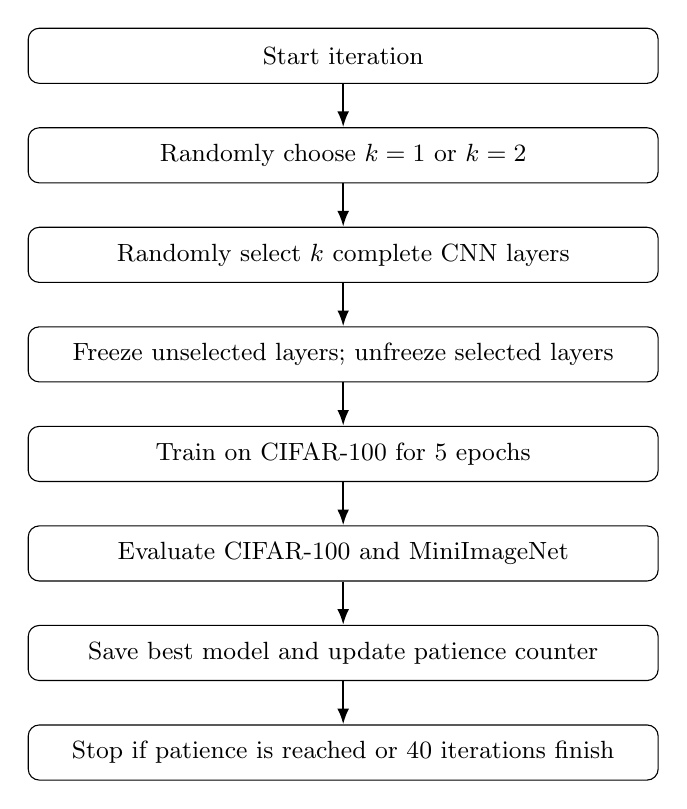
\begin{tikzpicture}[
    node distance=0.55cm,
    box/.style={draw,rounded corners,align=center,minimum width=8.0cm,
                minimum height=0.7cm,font=\small},
    arrow/.style={-{Latex[length=2mm]},thick}
]
\node[box] (a) {Start iteration};
\node[box,below=of a] (b) {Randomly choose $k=1$ or $k=2$};
\node[box,below=of b] (c) {Randomly select $k$ complete CNN layers};
\node[box,below=of c] (d) {Freeze unselected layers; unfreeze selected layers};
\node[box,below=of d] (e) {Train on CIFAR-100 for 5 epochs};
\node[box,below=of e] (f) {Evaluate CIFAR-100 and MiniImageNet};
\node[box,below=of f] (g) {Save best model and update patience counter};
\node[box,below=of g] (h) {Stop if patience is reached or 40 iterations finish};
\draw[arrow] (a)--(b);
\draw[arrow] (b)--(c);
\draw[arrow] (c)--(d);
\draw[arrow] (d)--(e);
\draw[arrow] (e)--(f);
\draw[arrow] (f)--(g);
\draw[arrow] (g)--(h);
\end{tikzpicture}
\caption{DLA iterative procedure.}
\label{fig:dla}
\end{figure}

\section{GWA: Guided Weight Adaptation}
GWA selects approximately ten percent of the parameter elements
independently within each ResNet-18 stage. For a stage containing
$N_i$ parameter elements, the number selected is
\[
K_i=\max\left(1,\left\lfloor 0.10N_i\right\rfloor\right).
\]
A random permutation is generated for each stage, and the first
$K_i$ indices are selected. These indices are converted into binary
masks having the same shapes as their corresponding parameter tensors.

For a parameter tensor $\theta_i$, its binary mask is
$M_i\in\{0,1\}^{\mathrm{shape}(\theta_i)}$. During backpropagation,
the gradient is masked:
\[
\nabla_{\theta_i}^{\,\mathrm{masked}}\mathcal{L}
=
M_i\odot\nabla_{\theta_i}\mathcal{L}.
\]
Consequently, only the selected parameter elements receive non-zero
gradients from the masked update. A fresh set of masks is generated at
the beginning of each iteration. The CIFAR-100 classifier remains
fully trainable.

\begin{figure}[H]
\centering
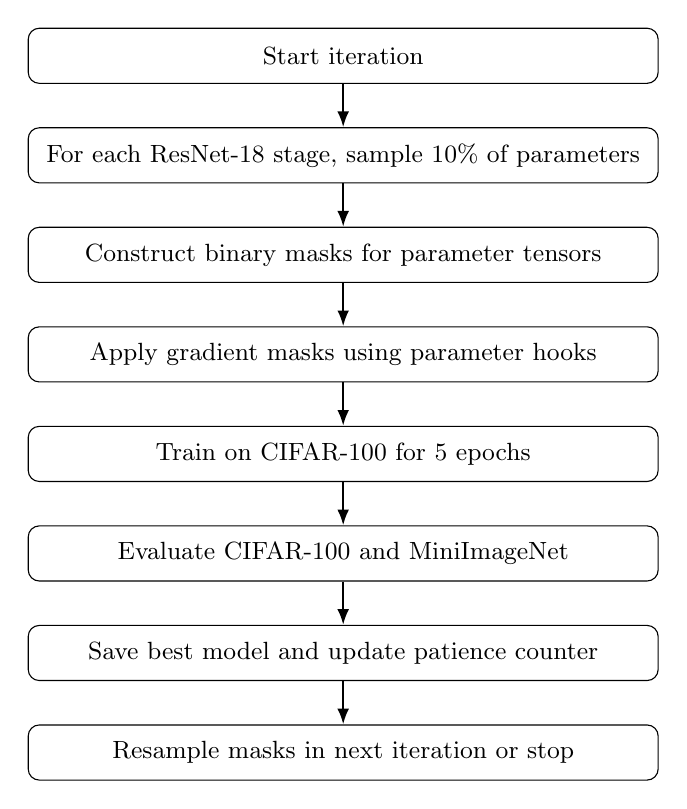
\begin{tikzpicture}[
    node distance=0.55cm,
    box/.style={draw,rounded corners,align=center,minimum width=8.0cm,
                minimum height=0.7cm,font=\small},
    arrow/.style={-{Latex[length=2mm]},thick}
]
\node[box] (a) {Start iteration};
\node[box,below=of a] (b) {For each ResNet-18 stage, sample 10\% of parameters};
\node[box,below=of b] (c) {Construct binary masks for parameter tensors};
\node[box,below=of c] (d) {Apply gradient masks using parameter hooks};
\node[box,below=of d] (e) {Train on CIFAR-100 for 5 epochs};
\node[box,below=of e] (f) {Evaluate CIFAR-100 and MiniImageNet};
\node[box,below=of f] (g) {Save best model and update patience counter};
\node[box,below=of g] (h) {Resample masks in next iteration or stop};
\draw[arrow] (a)--(b);
\draw[arrow] (b)--(c);
\draw[arrow] (c)--(d);
\draw[arrow] (d)--(e);
\draw[arrow] (e)--(f);
\draw[arrow] (f)--(g);
\draw[arrow] (g)--(h);
\end{tikzpicture}
\caption{GWA iterative procedure.}
\label{fig:gwa}
\end{figure}

\section{Training Procedure and Early Stopping}
Both supplied scripts follow an iterative training process. At the
beginning of each iteration, the trainable subset is selected. The
model is then trained on CIFAR-100 for five epochs. After training,
CIFAR-100 and MiniImageNet metrics are computed. The scripts track the
best CIFAR-100 accuracy and save the corresponding model state.

If CIFAR-100 accuracy does not improve for three consecutive
iterations, early stopping is triggered. The maximum number of
iterations is forty. Batch-normalization running statistics are kept
frozen during training in the supplied implementations.

\section{Evaluation Metrics}
\subsection{CIFAR-100 Accuracy}
CIFAR-100 accuracy measures the percentage of target test examples
classified correctly:
\[
A_{\mathrm{CIFAR}}=
\frac{\text{Number of correct CIFAR predictions}}
{\text{Total CIFAR test examples}}\times100.
\]

\subsection{MiniImageNet Accuracy}
MiniImageNet accuracy measures the percentage of MiniImageNet examples
classified correctly by the ImageNet evaluation head:
\[
A_{\mathrm{Mini}}=
\frac{\text{Number of correct MiniImageNet predictions}}
{\text{Total MiniImageNet examples}}\times100.
\]

\subsection{KL Divergence}
The scripts compare the output distributions of the initial reference
model and the updated model. The reported direction is
\[
D_{\mathrm{KL}}(P_{\mathrm{ref}}\Vert P_{\mathrm{updated}})
=
\sum_i P_{\mathrm{ref}}(i)
\log\frac{P_{\mathrm{ref}}(i)}{P_{\mathrm{updated}}(i)}.
\]
A smaller value indicates that the updated output distribution is
closer to the reference output distribution.

\subsection{Prediction Agreement}
Prediction agreement measures the fraction of examples for which the
initial and updated models predict the same class:
\[
\mathrm{Agreement}=
\frac{\sum_{n=1}^{N}
\mathbb{1}[\hat y_n^{\,\mathrm{ref}}=
\hat y_n^{\,\mathrm{updated}}]}{N}\times100.
\]
Agreement measures consistency with the reference model; it is not
the same as ground-truth classification accuracy.

\chapter{Results and Discussion}

\section{Comparative Results}
The project presentation records the following comparative values.

\begin{table}[H]
\centering
\caption{Comparative results recorded in the project presentation}
\label{tab:results}
\begin{tabular}{lrrrr}
\toprule
\textbf{Method} & \textbf{MB (\%)} & \textbf{MA (\%)} &
\textbf{CB} & \textbf{CA (\%)}\\
\midrule
DLA & 64.17 & 60.03 & 0.79 & 76.37\\
GWA & 66.53 & 63.42 & 0.79 & 75.96\\
\bottomrule
\end{tabular}
\end{table}

Here, MB denotes MiniImageNet accuracy before adaptation, MA denotes
MiniImageNet accuracy after adaptation, CB denotes the prediction
agreement value as recorded in the presentation, and CA denotes
CIFAR-100 accuracy. The presentation reports that both methods obtain
approximately 76\% CIFAR-100 accuracy and a prediction-agreement value
of approximately 79\%.

\textbf{Result provenance and consistency note:} The values above are
transcribed from the supplied presentation. The supplied code files
do not include the corresponding generated result CSV files, so these
values have not been independently recomputed from logs in this report.
Also, the supplied DLA code uses a randomly initialized custom CNN,
whereas the supplied GWA code uses pretrained ResNet-18. The presentation
describes a ResNet-18 primary architecture for the comparison. The
architecture and initialization used to generate the presentation
table must therefore be confirmed before treating the table as a
controlled head-to-head comparison.

\section{Discussion}
The reported table shows that DLA has a CIFAR-100 accuracy of 76.37\%,
while GWA has 75.96\%. GWA has a reported post-adaptation MiniImageNet
accuracy of 63.42\%, compared with 60.03\% for DLA. Both methods have
the same reported prediction agreement value of 0.79.

These values suggest that both parameter-selection strategies can
achieve useful target-task accuracy in the reported experiment.
However, a rigorous conclusion about which method better prevents
forgetting requires identical backbone architectures, identical
initialization, identical evaluation heads, and the same data splits.
The random initialization in the supplied DLA implementation is
particularly important: its frozen random ImageNet probe does not
provide a meaningful measure of preservation of pretrained ImageNet
knowledge.

\section{Ablation Study}
The project investigates several design choices that affect the
parameter-update process.

\subsection{Layer-Level and Weight-Level Selection}
DLA performs coarse-grained selection by enabling all parameters in
one or two complete layers. GWA performs fine-grained selection by
enabling approximately ten percent of the parameter elements in each
stage. These represent two different levels of update sparsity.

\subsection{Fresh Selection at Every Iteration}
Both algorithms generate a new trainable subset at each iteration.
For DLA, new complete layers are sampled. For GWA, new parameter masks
are generated independently for each stage. Resampling changes which
parameters can be updated over the course of training.

\subsection{Early Stopping}
The supplied implementations stop when CIFAR-100 accuracy fails to
improve for three consecutive iterations. This limits additional
training after the target accuracy has stopped improving. The stopping
criterion is based on CIFAR-100 accuracy and does not directly optimize
MiniImageNet retention.

\subsection{Limitations}
The current experimental setup has limitations that should be
considered when interpreting the results:
\begin{itemize}
    \item The supplied DLA and GWA code use different architectures
    and different initialization procedures.
    \item The DLA code initializes its custom CNN and its ImageNet
    evaluation probe randomly; therefore, its MiniImageNet accuracy
    cannot establish preservation of pretrained ImageNet knowledge.
    \item The reported presentation table is not accompanied by the
    raw experiment output files in the supplied materials.
    \item Prediction agreement measures similarity to the reference
    model's predictions and does not by itself prove that the updated
    model is correct.
    \item The early-stopping condition monitors CIFAR-100 accuracy,
    rather than directly balancing target accuracy and forgetting.
\end{itemize}

\chapter{Conclusion and Future Work}

\section{Conclusion}
This project studied two dynamic parameter-selection strategies for
neural-network adaptation: Dynamic Layer Adaptation and Guided Weight
Adaptation. DLA selects one or two complete layers of a four-layer CNN
at each iteration, while GWA selects approximately ten percent of
parameter elements independently within each stage of a pretrained
ResNet-18 and restricts gradients through binary masks.

The supplied implementations train on CIFAR-100 and evaluate on
MiniImageNet using accuracy, KL divergence, and prediction agreement.
The project presentation reports CIFAR-100 accuracies of 76.37\% for
DLA and 75.96\% for GWA, with approximately 79\% prediction agreement
for both. These results motivate further investigation of dynamic
parameter selection as a way to control model updates during
adaptation.

A fair conclusion about catastrophic-forgetting prevention requires
the two methods to be evaluated with the same pretrained backbone,
the same reference classifier, and the same evaluation protocol.
In particular, the current custom-CNN DLA implementation should be
modified to use a valid pretrained reference model and a meaningful
frozen evaluation head before its MiniImageNet retention can be
compared directly with GWA.

\section{Future Work}
The following directions can improve the current study:
\begin{itemize}
    \item Implement DLA and GWA on the same pretrained backbone to
    ensure a controlled comparison.
    \item Use the same pretrained reference model and frozen
    evaluation classifier for both methods.
    \item Investigate sensitivity-based or importance-based selection
    instead of purely random layer or parameter selection.
    \item Compare different selection ratios, including 5\%, 10\%,
    20\%, and 50\% of parameters.
    \item Study the effect of selecting one, two, or more complete
    layers in DLA.
    \item Incorporate knowledge distillation or replay-based learning
    to improve retention of the original domain.
    \item Evaluate on additional datasets and architectures to study
    generalization.
    \item Report multiple random seeds, confidence intervals, and
    complete training histories for statistically stronger results.
    \item Develop a stopping criterion that considers both target
    accuracy and reference-domain performance.
\end{itemize}

% =========================================================
% REFERENCES
% =========================================================
\begin{thebibliography}{99}

\bibitem{ewc}
J. Kirkpatrick et al., ``Overcoming catastrophic forgetting in neural
networks,'' \emph{Proceedings of the National Academy of Sciences},
vol. 114, no. 13, pp. 3521--3526, 2017.

\bibitem{packnet}
A. Mallya and S. Lazebnik, ``PackNet: Adding multiple tasks to a
single network by iterative pruning,'' in \emph{Proceedings of the
IEEE Conference on Computer Vision and Pattern Recognition (CVPR)},
2018.

\bibitem{progressive}
A. A. Rusu et al., ``Progressive neural networks,'' arXiv:1606.04671,
2016.

\bibitem{lora}
E. J. Hu et al., ``LoRA: Low-rank adaptation of large language models,''
in \emph{International Conference on Learning Representations (ICLR)},
2022.

\bibitem{adapters}
N. Houlsby et al., ``Parameter-efficient transfer learning for NLP,''
in \emph{Proceedings of the 36th International Conference on Machine
Learning (ICML)}, 2019.

\bibitem{lottery}
J. Frankle and M. Carbin, ``The lottery ticket hypothesis: Finding
sparse, trainable neural networks,'' in \emph{International Conference
on Learning Representations (ICLR)}, 2019.

\end{thebibliography}

\end{document}
